
All News,Blogs and Tweets are first filtered by searching for the 
presence of at least one key phrase which indicate indicate that the document might be about a planned future event. 
The filtered documents are then searched for the mention of a future date. In case of News/blogs, 
the search for future date mentions is restricted to the sentence in which the keyphrase was found.
where the phrase was found to reduce error. For tweets, no such restriction is made.

A warning/alert is then finally issued for those documents which also contain any location information.
In the case of tweets, to avoid false alarms, we further filter the tweets by setting a threshold (set to 5) on the number of re-tweet of the tweet under consideration.  Event type information and population information is derived from the text of the document.  

In the case of Facebook, a Facebook-Event is considered an alert if there are more number of attendees than number of rejects.

\begin{figure*}
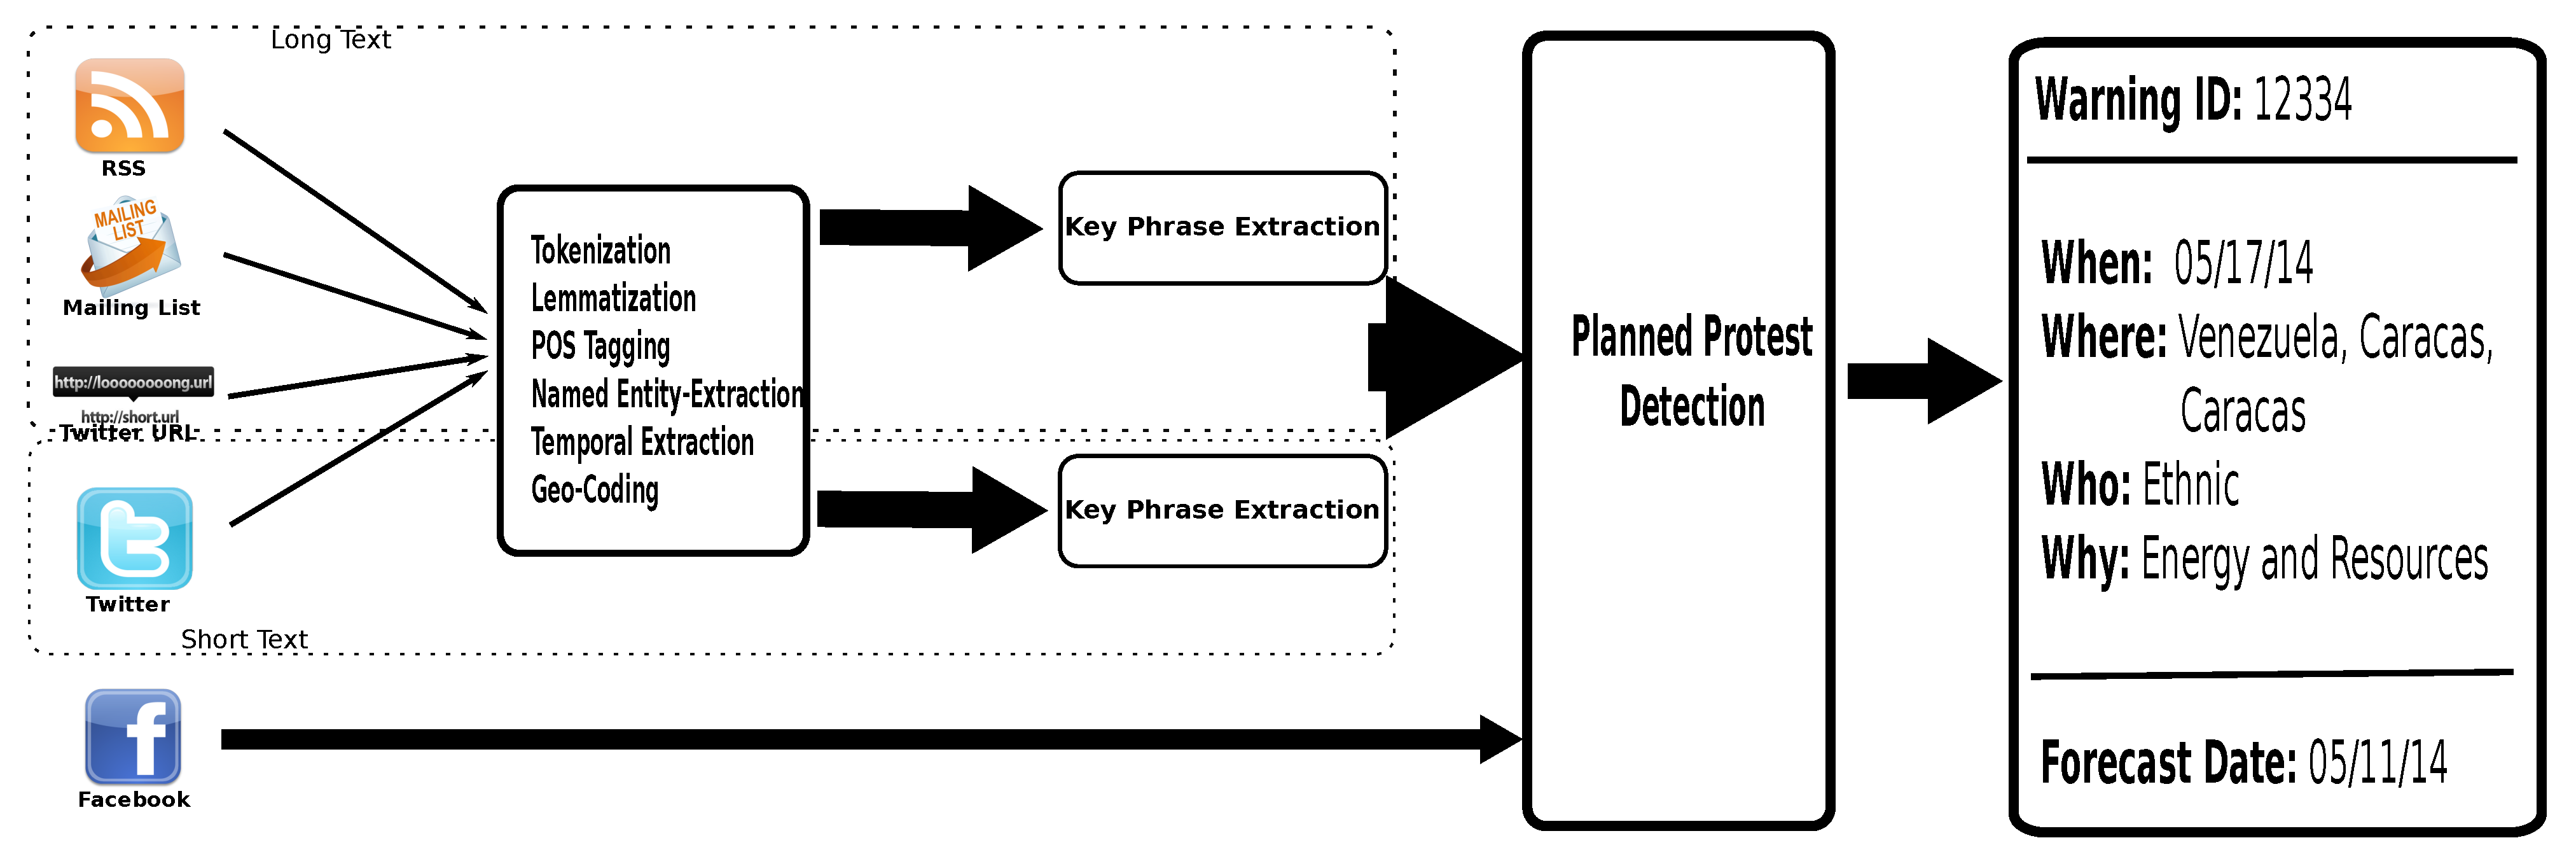
\includegraphics[width=\textwidth]{pp_pipeline}
\caption{A diagram showing various steps of the Model}
\end{figure*}

\subsection{Phrase filtering}

Each input message (document) is searched for the presence of one or
more key phrases in a list of phrases indicative of an article's being
about a planned civil unrest event.  Articles which do match are sent on for further processing,
and those that do not are ignored, again, as part of the streaming infrastructure.

The list of key phrases indicating civil unrest planning was obtained
in a semi-automatic manner, as detailed in the following section. The
phrases are general rules for matching, rather than literal string
sequences, typically consisting of two or more word lemmas, a language
specification and a separation threshold. This separation threshhold is automatically learned
in the learning phrase described below.  It was found that this kind of multi-word key phrases was found more accurate than simple
keywords for extracting events of interest from the data stream.

The presence of a keyphrase is checked by searching for the presence of
individual lemmas of the keyphrase within the same sentence separated
by at most a number of word that is fewer than the separation threshold.  
This method allows for linguistically sophisticated and flexible matching, so, for example,
they keyphrase [{\em plan protest}, 4, English] would match the sentence
{\em The students are planning a couple big protests tomorrow} in an input document.


\subsubsection{Phrase list development}
\label{sec:phraselearning}

We make use of a semi-automated approach to identify key-phrases for the purpose of extracting events from our data feeds. We use different sets of phrases for News and Twitter. We found that key-phrases provide a more accurate extraction than individual keywords.

Initially, a few seed phrases were obtained manually
with the help of subject matter experts. These phrases were parsed
using a dependency parser and the grammatical relationship between the
core subject word---{\em protest}, {\em manifestación}, {\em Huelga},
etc.---and any accompanying word -- {\em plan}, {\em call}, {\em anunciar} --- was extracted. These grammatical relations serve as extraction patterns as in \cite{riloff2003learning}. Then, we build a corpora by finding out sentences that contain both a future date and the protest or its synonyms in any of the three languages. These sentences are then used as candidates for phrase list expansion. The phrase list is populated by finding phrases that follows the extraction pattern.
The phrase learning is shown in Fig.~/ref{fig:phraselearning}

This final set of phrases, is then cleansed by an expert to get the final set of phrases. Around 122 phrases were obtained for News/Blogs and 

To extend the initial set of phrases, a set of sentences/tweets containing a subject word and a
future time/date expression was collected and parsed.  This set of
sentences was used to expand the set of planned protest phrases by
extracting all keyword combinations that have the same grammatical
relation with respect to the core subject word. The final set of
planned protest phrases is then obtained after a manual revision of
the phrases obtained in the last step.

By this approach, we learned 112 phrases for News/blogs and 156 for tweets.

The learned phrases are then used to filter the incoming stream of Documents (news/blogs/twitter). The phrases matching is done by first splitting the incoming document into sentences and then looking for the presence of each individual word of a key-phrase (by lemma) separated by a pre-fixed maximum offset-distance (set to 3). This methodology greatly increases processing speed.

\begin{figure}
\caption{An Example of Phrase Learning}
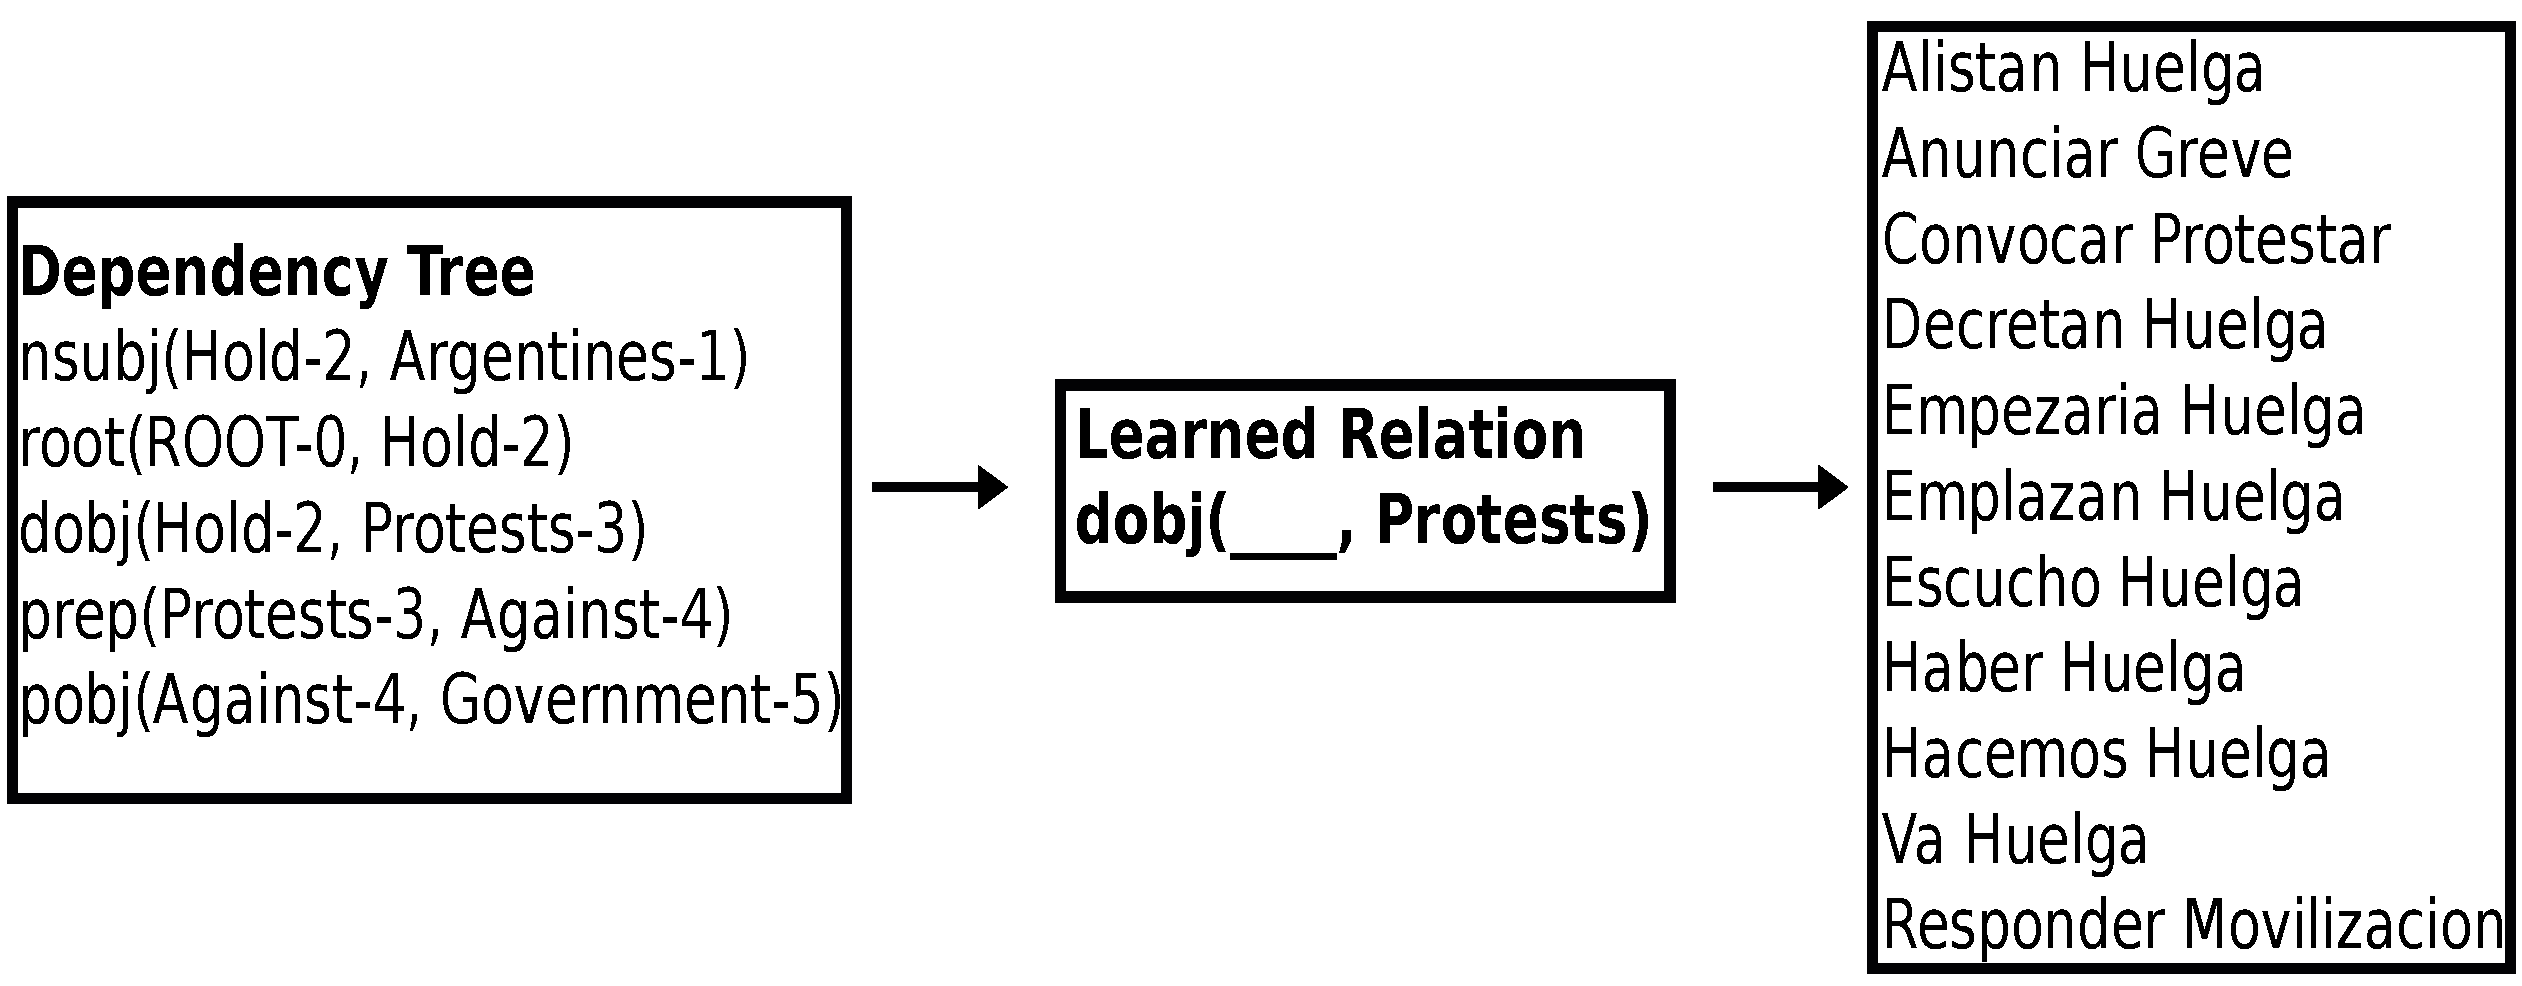
\includegraphics[width=0.5\textwidth]{figures/phraseLearning}
\label{fig:phraseLearning}
\end{figure}


The set of key phrases was tailored (slightly) the the genre of the
input. In particular different phrases were used to identify relevant
news articles and blogs from those used to filter Tweets.  The lists
themselves were generated semi-audomatically.

Initially, a few seed phrases were obtained manually
with the help of subject matter experts.
\sathappanc{Jaime's Text --> edited by graham}
An analysis of news reports for planned protests in the print media helped create a
minimum set of words to use in the query.  We choose four nouns from
the basic query that is used predominantly to indicate a civil unrest
in the print media - {\em demonstration, march, protest and
  strike}. We translated them into Spanish and Portuguese, including
synonyms.  We then combined these with future-oriented verbs - {\em to organize}, {\em to prepare}, {\em to
plan}, {\em to announce}, etc. For twitter, shorter phrases were identified, and these had
a more direct call for action, for example, {\em marchar}, {\em manhã de mobilização}, {\em
  vamos protestar}, {\em huelga}.

To generalize this set of phrases, the the phrases were then parsed
using a dependency parser \cite{freeling} and the grammatical
relationship between the core the nominal focus word (e.g., {\em
  protest}, {\em manifestación}, {\em huelga}) and any accompanying
word (e.g., {\em plan}, {\em call}, {\em anunciar}) was
extracted. These grammatical relations were used as extraction
patterns as in \cite{riloff2003learning} to learn more phrases from a
corpora of sentences extracted from the data stream of interest
(either news/blogs or tweets). This corpus consists of sentences that
contained any one of the nominal focus words and also had mentions of a
future date.

The phrase learning is shown in Fig.~\ref{fig:phraselearning}

The set of learned phrases, is then cleansed by an expert to get the final set of key phrases.
Using this approach, we learned 112 phrases for news articles andblogs and 156 for tweets.

\begin{figure}
\caption{An Example of Phrase Learning}
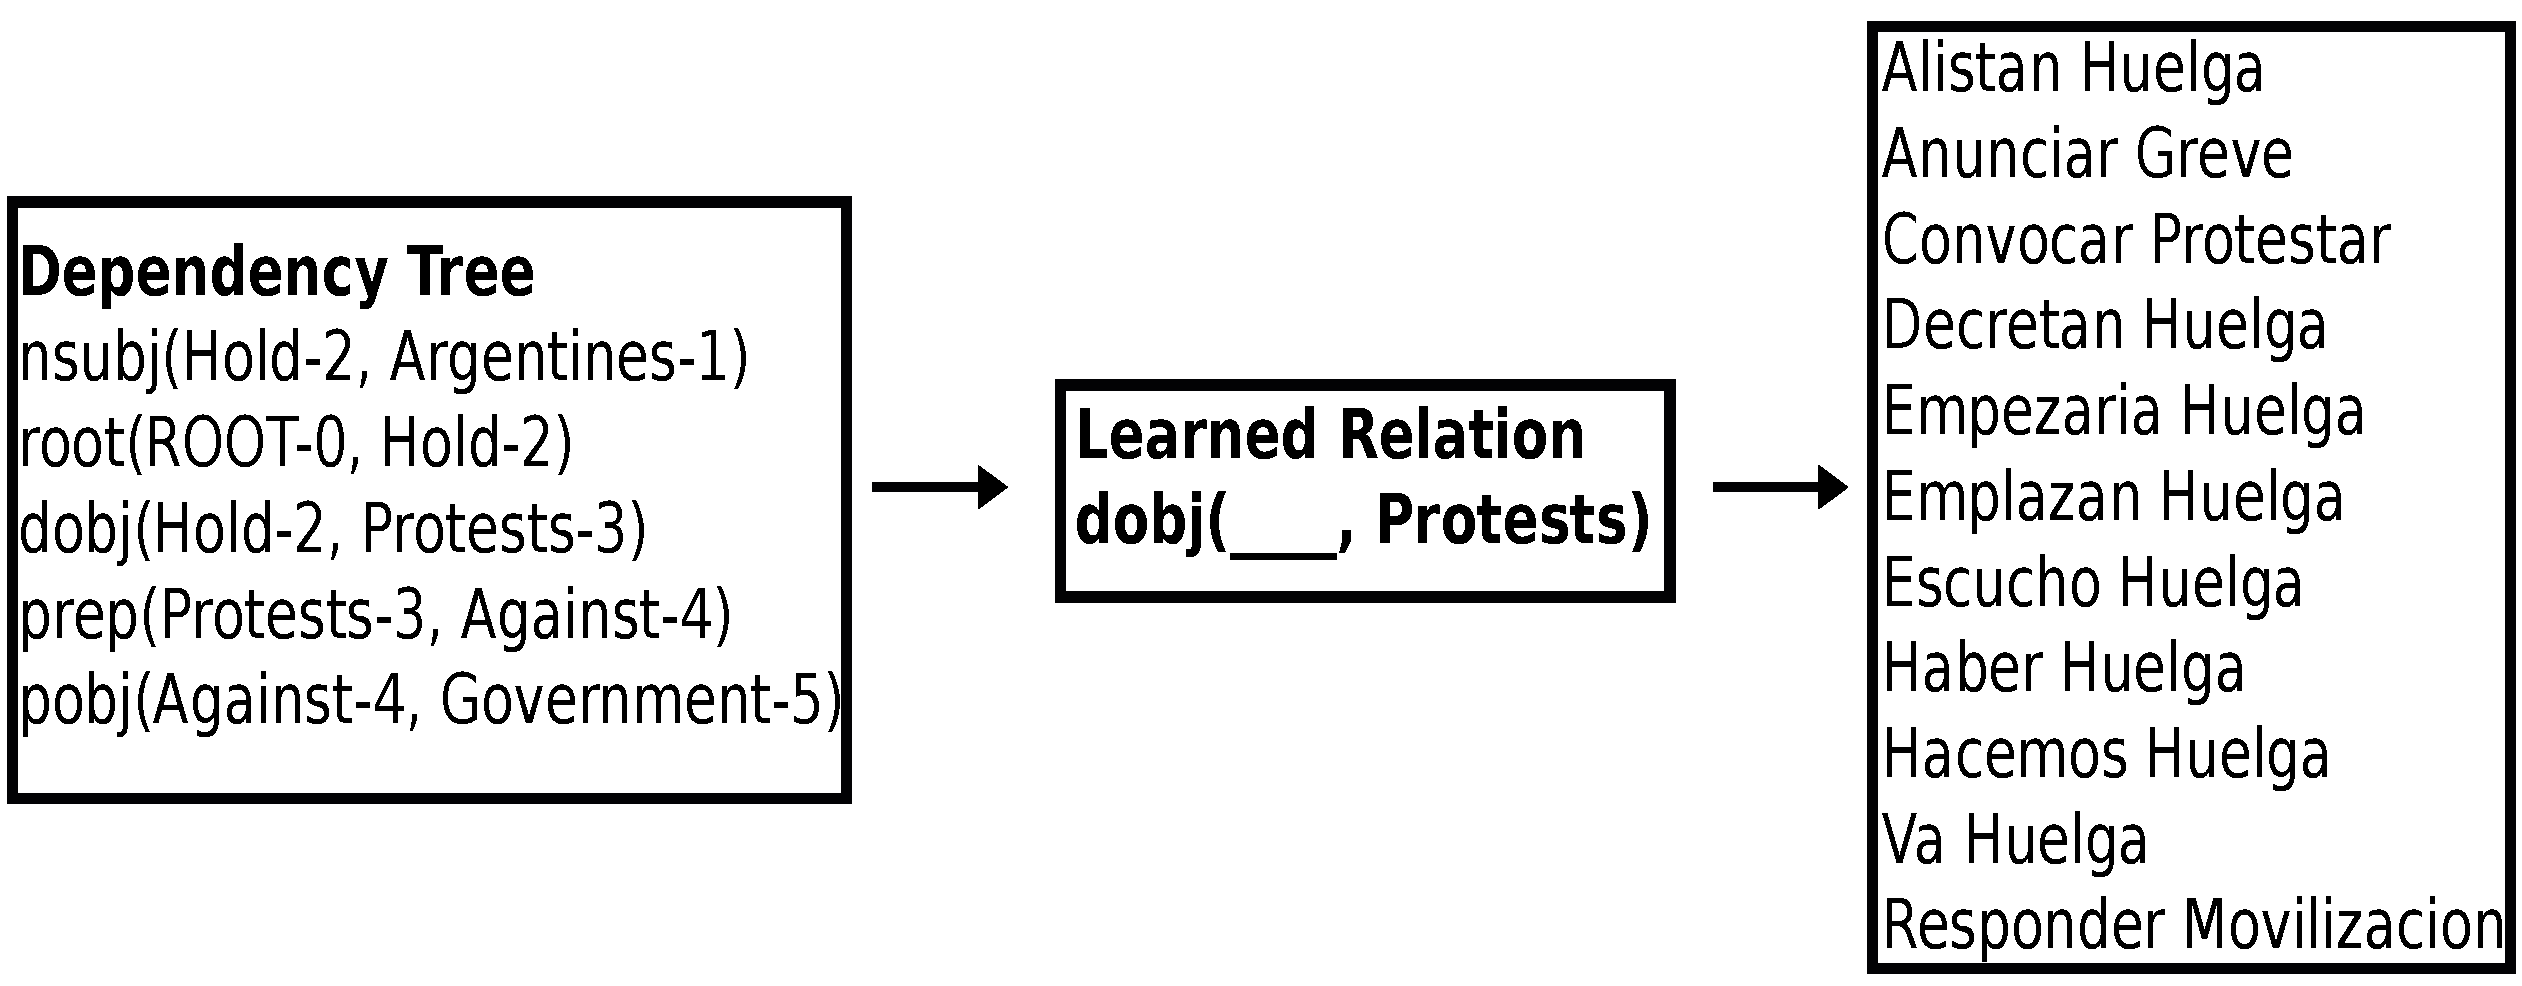
\includegraphics[width=0.5\textwidth]{figures/phraseLearning}
\label{fig:phraselearning}
\end{figure}


\subsection{classification}

For News/Blogs and Facebook, we make use of Text Based Naive Bayes
Classifier to identify the event-type and population. Unigram and
Bi-gram word features are used for training the classifier.

For Twitter, as we send alerts based on a single tweet, we chose the
event-type and population based on prior likelihood for that location.

